%%%%%%%%%%%%%%%%%%%%%%%%%%%%%%%%%%%%%%%%%%%%%%%%%%%%%%%%%%%%%%%%%%%%%%%%%%%%%%%%%%%%%%%%%%%%%%%%%%%%%%%%%%%%%%%%%%%%%%%%%%%%%%%%%%%%%%%%%%%%%%%%%%%%%%%%%%%%%%%%%%%%%%%%%%%%%%%%%%%%
\FloatBarrier
\chapter{Motivation}
\label{sec:Motivation}
Supersymmetry is able to offer solutions to many unexplained phenomena in astrophysics and can solve many of the shortcomings of the Standard Model of particle physics (see Section~\ref{FIXME}).
While SUSY has been studied at previous particle colliders including Tevatron and LEP~\cite{bib:Tevatron:SUSY_results,bib:LEP:SUSY_results}, the LHC with its high centre-of-mass energy offers a unique opportunity to investigate SUSY models with high sparticle masses that were not accessible in previous experiments.

Therefore, a variety of searches were hunting for SUSY during Run\,I of the LHC in 2011 and 2012.
Proton-proton collision data from the CMS and ATLAS experiments were analysed with a strong focus on the search for SUSY in the strong production sector (\eg~\cite{bib:CMS:RA2_8TeV,bib:CMS:MT2_8TeV,bib:ATLAS:JetPlusMET_8TeV}).
As a consequence, wide, previously unexplored regions of SUSY parameter space are already excluded.
However, due to the unknown mechanism of supersymmetry breaking, the most general parametrisation of the Minimal Supersymmetric Standard Model (MSSM) introduces over 100 new parameters and thus opens up an incredibly large phenomenological space. 
Therefore, SUSY models can lead to a plethora of possible signatures at particle colliders, many of which could not - or not fully - be explored. \\

%Among more ``exotic'' SUSY scenarios are models with compressed spectra, where two or more particles are nearly mass-degenerate.
%Especially scenarios with a nearly mass-degenerate lightest chargino (\chipm) and lightest neutralino (\chiO) are very interesting from a theoretical and cosmological perspective as they can help to explain the sources of the relic den%sity~\cite{bib:Moroi:DarkMatter_1999,bib:Hisano:DarkMatter_2005,bib:Ibe:DarkMatter_2015}.
%While it is not possible to explain the full relic density with thermally produced neutralinos for m$_{\chiO}\lesssim 2.9\tev$~\cite{bib:Moroi:DarkMatter_2013}, neutralinos can still be the dominant part if they are non-thermally produ%ced via the decay of a long-lived particle such as a wino-like chargino.
%The enhanced annihilation cross section (called Sommerfeld enhancement) into $WW$- , $ZZ$- or $ff$-pairs for a wino-like dark matter candidate leads to an underprediction of the relic density if the neutralino and chargino masses are t%oo small~\cite{bib:Hisano:DarkMatter_2003}.
%This underprediction can be cured, however, if there is an additional non-thermal production of dark matter that is caused by the decay of a long-lived chargino.
%In Supersymmetry, such a mass-degeneracy naturally occurs in case of wino-like neutralinos and charginos, since the mass gap between $W_{3}$ and $W_{1/2}$ is fully determined by higher loop corrections (see Section~\ref{FIXME}).

%Among more ``exotic'' SUSY scenarios are models with compressed spectra, where two or more particles are nearly mass-degenerate.
%Especially scenarios with a wino-like 
%Especially scenarios with a nearly mass-degenerate lightest chargino (\chipm) and lightest neutralino (\chiO) are very interesting from a theoretical and cosmological perspective as they can help to explain the sources of the relic den%sity~\cite{bib:Moroi:DarkMatter_1999,bib:Hisano:DarkMatter_2005,bib:Ibe:DarkMatter_2015}.
%While it is not possible to explain the full relic density with thermally produced neutralinos for m$_{\chiO}\lesssim 2.9\tev$~\cite{bib:Moroi:DarkMatter_2013}, neutralinos can still be the dominant part if they are non-thermally produ%ced via the decay of a long-lived particle such as a wino-like chargino.
%The enhanced annihilation cross section (called Sommerfeld enhancement) into $WW$- , $ZZ$- or $ff$-pairs for a wino-like dark matter candidate leads to an underprediction of the relic density if the neutralino and chargino masses are t%oo small~\cite{bib:Hisano:DarkMatter_2003}.
%This underprediction can be cured, however, if there is an additional non-thermal production of dark matter that is caused by the decay of a long-lived chargino.
%In Supersymmetry, such a mass-degeneracy naturally occurs in case of wino-like neutralinos and charginos, since the mass gap between $W_{3}$ and $W_{1/2}$ is fully determined by higher loop corrections (see Section~\ref{FIXME}).

A very interesting signature occurs when sparticles live long enough to travel through a part or the whole detector before decaying.
%Among these are very interesting signatures where sparticles live long enough to travel through a part or the whole detector before decaying.
This is possible for SUSY models with compressed spectra, in which a sparticle can be long-lived because of phase-space suppression (see Section~\ref{sec:FIXME.Theory:Lifetimes}).
%Among more ``exotic'' SUSY scenarios are models with compressed spectra, where two or more particles are nearly mass-degenerate.
In Supersymmetry, such a mass-degeneracy naturally occurs if the wino mass parameter ($M_2$) is much smaller than the bino ($M_1$) and higgsino ($\mu$) mass parameters.
In this case, the lightest chargino (\chipm) and the lightest neutralino (\chiO) are both wino-like and their mass gap is fully determined by higher loop corrections (see Section~\ref{FIXME}).
Therefore, they are almost mass-degenerate and the chargino is long-lived.

Such scenarios can be very interesting from a cosmological perspective as the wino-like lightest supersymmetric particle, \chiO, can serve as a plausible Dark Matter candidate~\cite{bib:Hisano:DarkMatter_2005,bib:Ibe:DarkMatter_2015}.
%Such scenarios lead to a very interesting collider phenomenology and due to the wino-like lightest supersymmetric particle, \chiO, include a plausible Dark Matter candidate~\cite{bib:Hisano:DarkMatter_2005,bib:Ibe:DarkMatter_2015}.
While it is not possible to explain the full relic density with thermally produced wino-like neutralinos for m$_{\chiO}\lesssim 3\tev$, neutralinos can still be the dominant part if they are non-thermally produced via the decay of an almost decoupled particle~\cite{bib:Moroi:DarkMatter_1999,bib:Moroi:DarkMatter_2013}.
Additionally, these scenarios are well motivated by Supersymmetric models with anomaly-mediated SUSY breaking (AMSB)~\cite{bib:Theory_AMSB_1998,bib:Theory_AMSB_1999}, where the LSP is almost always the wino-like lightest neutralino and the mass gap between the neutralino and chargino is typically between 140\mev and 200\mev~\cite{bib:Theory_MassGap_2014}. \\
%The enhanced annihilation cross section (called Sommerfeld enhancement) into $WW$- , $ZZ$- or $ff$-pairs for a wino-like dark matter candidate leads to an underprediction of the relic density if the neutralino mass is too small~\cite{bib:Hisano:DarkMatter_2003}.
%This underprediction can be cured, however, if there is an additional non-thermal production of dark matter as explained before.

SUSY scenarios with nearly mass-degenerate particles have two distinctive phenomenological properties that require a very different search strategy compared to general SUSY searches. 
First, because of the mass-degeneracy, the remaining decay product (\eg a pion) is very soft in \pt, making it hard to detect.
Since the other decay product, the neutralino, is only weakly interacting, it is very difficult to identify charginos via their decay products. 
% makes the detection of the chargino by the decay products a challenging task. 
%First, if the chargino and the neutralino are almost mass-degenerate, the remaining decay product (\eg a pion) is very soft in \pt, making it hard to detect.
Second, as the chargino is long-lived, it may traverse several detector layers before decaying.
Thus, there is the possibility of reconstructing the chargino itself, \eg as a reconstructed track in the tracker system.
%However, how the chargino is reconstructed is highly dependent on its concrete lifetime.
%However, depending on the concrete lifetime of the chargino, the reconstruction of the chargino this reconstruction can require very different tools compared to the reconstruction of Standard Model particles.
 \\

%Even though supersymmetric models with nearly mass-degenerate \chipm and \chiO lead to exotic signatures with long-lived charginos and soft decay products, current CMS searches are already sensitive over a very broad range of lifetimes.

Despite the exotic signatures of supersymmetric models with nearly mass-degenerate \chipm and \chiO, current CMS searches are already sensitive over a very broad range of lifetimes.
The exclusion power of existing SUSY searches can be assessed by interpreting their results in terms of the fraction of excluded parameter points in the phenomenological MSSM (see Section~\ref{theorySUSY} for an introduction to the pMSSM). 
The results of such a study which has been performed in \cite{bib:CMS:DT_8TeV} are shown in Figure~\ref{fig:pMSSMplot}. 
\begin{figure}[!t]
  \centering 
  \begin{tabular}{c}
    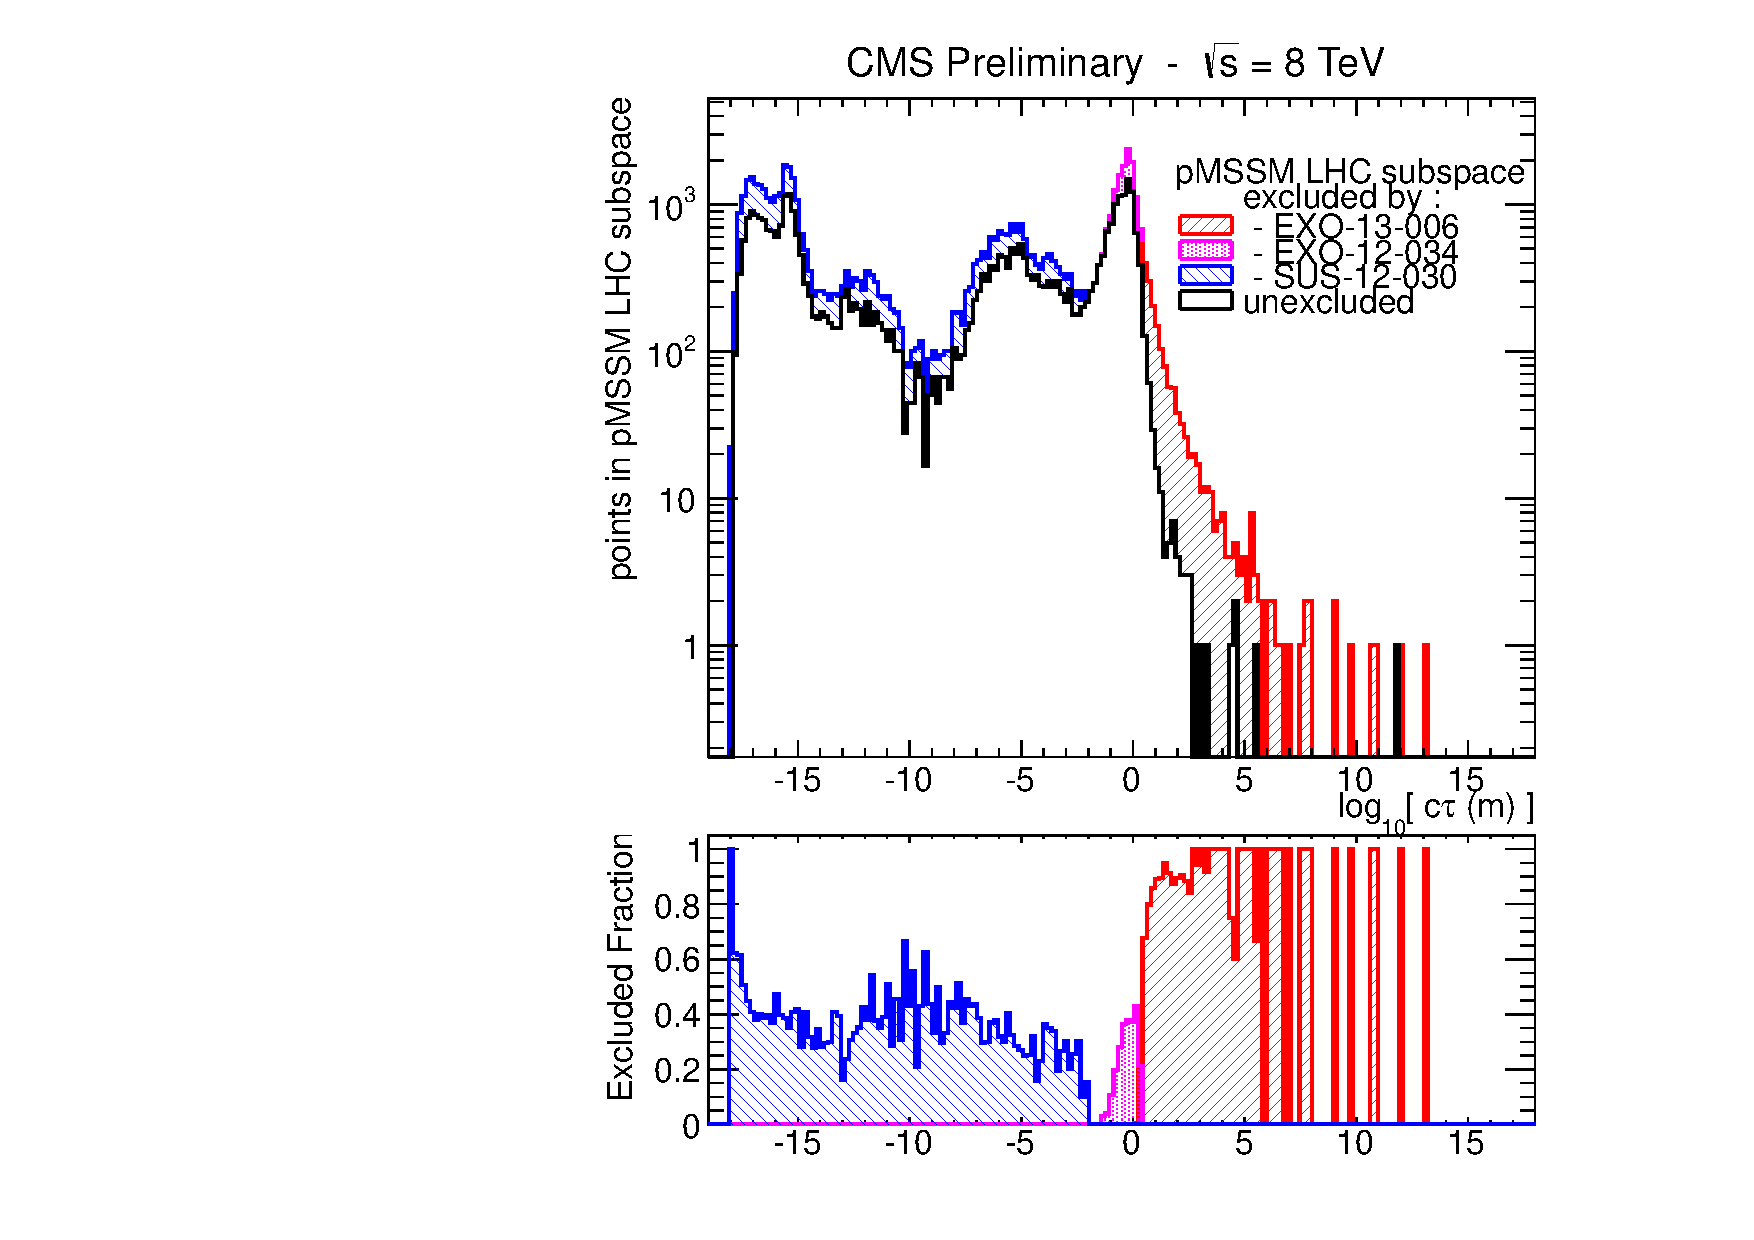
\includegraphics[width=0.75\textwidth]{figures/analysis/pMSSM_vs_ctau.pdf}
  \end{tabular}
  \caption{The number of excluded pMSSM points at 95\% C.L. (upper part) and the fraction of excluded pMSSM points (bottom part) vs. the chargino lifetime for different CMS searches.
           Red area: the search for long-lived charged particles \cite{bib:CMS:HSCP_8TeV},
           Purple area: the search for disappearing tracks  \cite{bib:CMS:DT_8TeV},
           Blue area: a collection of various general SUSY searches \cite{bib:CMS:pMSSMinterpretation_7TeV_PAS}
           The black line indicates the unexcluded pMSSM parameter points.
           The sampling of the parameter space points was done according to a prior probability density function which takes pre-LHC data and results from indirect SUSY searches into account (see \cite{bib:CMS:HSCPReinterpreation_PAS} for further details).
           Taken from: \cite{bib:pMSSMplot_source_from_DT}.}
  \label{fig:pMSSMplot}
\end{figure}
It can be seen that general SUSY searches (blue area) are sensitive to shorter chargino lifetimes ($c\tau \lesssim 10\cm$). 
Due to technical reasons\footnote{The pMSSM interpretation relied on the use of fast simulation techniques which are not capable of simulating charginos with lifetimes $\ctau>1\cm$.}, the general SUSY searches were never interpreted in the context of SUSY models with longer chargino lifetimes. 
Two existing searches, the search for long-lived charged particles~\cite{bib:CMS:HSCP_8TeV} and the search for disappearing tracks~\cite{bib:CMS:DT_8TeV} focus on long and intermediate chargino lifetimes, respectively. 
These two searches (purple and red areas) are sensitive to chargino lifetimes of $\ctau \gtrsim 35\cm$.
Taken together, the existing searches exclude a large fraction of pMSSM points at different chargino lifetimes. 
However, there is a gap between the general SUSY searches and the search for disappearing tracks that is not accessible by any of the existing searches.\\

The here presented analysis aims at targeting this gap by optimising the search strategy for charginos with intermediate lifetimes of $10\cm \lesssim c\tau \lesssim 40\cm$. 
The targeted optimisation strategy is a combination of the strategies used in the search for long-lived charged particles~\cite{bib:CMS:HSCP_8TeV} and the search for disappearing tracks~\cite{bib:CMS:DT_8TeV}.
While in~\cite{bib:CMS:HSCP_8TeV}, the high ionisation losses of hypothetical new massive particles is exploited, it does not take into account whether its reconstructed track is disappearing.
In~\cite{bib:CMS:DT_8TeV}, the disappearance of the track is utilised but it does not incorporate the large ionisation losses into the search.
Additionally, neither of the search does take into account the possibly very short tracks of early decaying charginos.\\

Thus, the here presented search is the first analysis at CMS combining the two signature properties that are highly distinctive for charginos with intermediate lifetimes: 
first, the characteristically high ionisation losses of heavy charginos;
second, short reconstructed tracks due to chargino decays early in the detector. 

The associated challenges and the general search strategy of this analysis will be presented in the next section.

%%%%%%%%%%%%%%%%%%%%%%%%%%%%%%%%%%%%%%%%%%%%%%%%%%%%%%%%%%%%%%%%%%%%%%%%%%%%%%%%%%%%%%%%%%%%%%%%%%%%%%%%%%%%%%%%%%%%%%%%%%%%%%%%%%%%%%%%%%%%%%%%%%%%%%%%%%%%%%%%%%%%%%%%%%%%%%%%%%%%
%%%%%%%%%%%%%%%%%%%%%%%%%%%%%%%%%%%%%%%%%%%%%%%%%%%%%%%%%%%%%%%%%%%%%%%%%%%%%%%%%%%%%%%%%%%%%%%%%%%%%%%%%%%%%%%%%%%%%%%%%%%%%%%%%%%%%%%%%%%%%%%%%%%%%%%%%%%%%%%%%%%%%%%%%%%%%%%%%%%%
